\documentclass{beamer}

\usetheme{GNURadio}
\usepackage{palatino}
\usepackage{xcolor}
\usepackage{tikz}
\usepackage[utf8]{inputenc}
\usepackage{listings}
\usepackage{alltt}

\title{PyBOMBS \& CGRAN --- An Introduction}
\institute{Martin Braun}

\date{GNU Radio Conference 2016}

\graphicspath{{./}}
\DeclareGraphicsExtensions{.png,.pdf}

% Comment this out to not have a TOC every time you have a \section:
\AtBeginSection[] {%
  \begin{frame}
    \frametitle{Outline}
    \tableofcontents[currentsection]
  \end{frame}
}

\begin{document}

% Title page:
\frame{\titlepage}

\section{How do I even get started with GNU Radio?}
\begin{frame}
  \frametitle{Let's assume for just one minute\ldots}
  \begin{itemize}
    \item \ldots{}that I have no idea how to get started with GNU Radio.
    \item<2-> I mean, I literally don't even know how to run the examples and tutorials.
    \item<3-> No worries. We've got you covered.
  \end{itemize}
\end{frame}

\begin{frame}
  \frametitle{Top 4 easiest ways to install GNU Radio}
  \begin{enumerate}
    \item The GNU Radio Live DVD
    \item<2-> \texttt{apt-get install gnuradio} --- use your package manager, whatever that is
    \item<3-> PyBOMBS
    \item<4-> Source Builds
  \end{enumerate}
    \hspace{3em}
    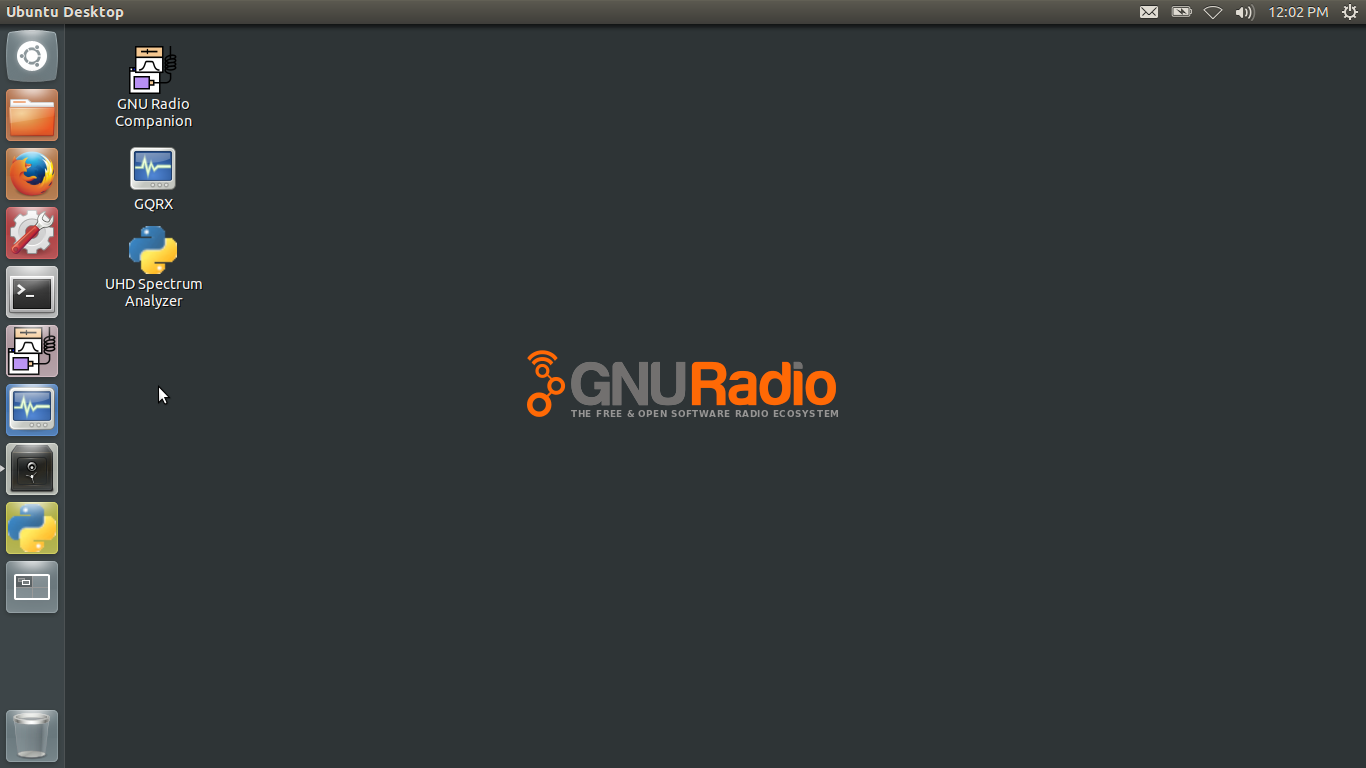
\includegraphics[height=5em]{grlivedvd}
    \hspace{1em}
    \includegraphics<3->[height=5em]{pybombs_logo}
    \hspace{1em}
    \includegraphics<4->[height=5em]{srcbuild}
\end{frame}

% Concepts:
% - Local prefix
% - 

\begin{frame}
  \frametitle{What you will need}
  \begin{itemize}
    \item A Linux or Mac box (one day we'll have Windows covered, but not today)
    \item Fedora, Ubuntu, CentOS, Debian, and probably many other distros fine
    \item Python 2.7
    \item<2-> And what else\ldots
    \item<3-> Nope, that's it!
  \end{itemize}
\end{frame}

\begin{frame}
  \frametitle{Getting started with PyBOMBS}
  \begin{itemize}
    \item Install PyBOMBS\@: \texttt{pip install pybombs}
    \item Optionally install PyBOMBS GUI\@: \texttt{pip install pybombs-qtgui}
    \item Next, run some magic commands that I'll skip for now.
    \item Let's just install GNU Radio and all major dependencies:
    \item \footnotesize{\texttt{pybombs prefix init -a default -R gnuradio-default /home/mbr0wn/prefix/gnuradio}}
    \item<2-> Whoa, slow down hot shot\ldots
  \end{itemize}
\end{frame}

\section{PyBOMBS concepts}
\begin{frame}
  \frametitle{Why do I need a \emph{prefix}?}
  \begin{itemize}
    \item Standard Unix way (since probably even Marcus Leech started) is to install software either into \texttt{/usr} or \texttt{/usr/local}.
    \item Self-compiled software would go into the latter
    \item This is simple and understood, but has some problems:
    \begin{itemize}
      \item No standard way to uninstall hand-installed software
      \item Only one installation at a time possible
      \item Always requires admin (sudo) privileges
    \end{itemize}
    \item So how about we install it into some random directory in our home?
    \item \texttt{/home/mbr0wn/prefix/gnuradio} --- The prefix!
    \item Solves all the problems above, except we now need to tell the system where to look for stuff (\emph{environment variables} need setting)
  \end{itemize}
\end{frame}

\begin{frame}
  \frametitle{\texttt{pybombs prefix init}}
  \begin{itemize}
    \item Show me that command again:
      \begin{alltt}
      pybombs\\
          prefix init \\
          --alias default \\
          --recipe gnuradio-default \\
          /home/mbr0wn/prefix/gnuradio
      \end{alltt}
    \item Aah, I get it now. We install into \texttt{prefix/gnuradio}, and we use the rules defined in \texttt{gnuradio-default}.
    \item We call such definitions a \emph{recipe}.
  \end{itemize}
\end{frame}

\begin{frame}
  \frametitle{So\ldots recipes?}
  \begin{itemize}
    \item Remember those magic commands I skipped? Here they are:
      {\footnotesize{%
\begin{alltt}
\$ pybombs recipes add gr-recipes  \\
git+https://github.com/gnuradio/gr-recipes.git \\
\$ pybombs recipes add gr-etcetera\\
git+https://github.com/gnuradio/gr-etcetera.git
\end{alltt}
}}
    \item These are part of most people's installation. (See PyBOMBS manual).
    \item Will install all default recipes.
    \item Let's take a quick look at one of those.
  \end{itemize}
\end{frame}

\begin{frame}
  \frametitle{How do I install things then?}
  \begin{itemize}
    \item \texttt{pybombs install [-p PREFIX ] PACKAGE}
    \item Let me show you.
    \item \texttt{PREFIX} is either an alias, or a full path.
  \end{itemize}
\end{frame}

\begin{frame}
  \frametitle{Why is PyBOMBS accessing my system?}
  \begin{itemize}
    \item PyBOMBS is not a container replacement.
    \item It will use any means to get your system ready to build software (e.g., GNU Radio).
    \item Your system's package manager is one of those means.
    \item It might need elevated privileges. This is normal.
    \item Here's a nice trick: \texttt{pybombs install --deps-only gnuradio}
  \end{itemize}
\end{frame}

\section{Out-of-tree Modules}
\begin{frame}
  \frametitle{But what is there to install?}
  \begin{itemize}
    \item You could browse the list of recipes.
    \item But let's have something nice instead!
    \item \texttt{www.cgran.org} FTW\@!
    \item Most the things listed on CGRAN are \emph{out-of-tree modules}.
  \end{itemize}
\end{frame}

\begin{frame}
  \frametitle{Out-of-tree Modules}
  \begin{itemize}
    \item GNU Radio comes with a lot of blocks, but a lot of the value comes from the ability to extend it.
    \item Other people like to share their extensions to GNU Radio!
    \item Side note: Making OOTs is really easy. Just use \texttt{gr\_modtool}!
  \end{itemize}
\end{frame}


%\section{Examples}
%\begin{frame}
  %\frametitle{Stuff}
  %\begin{block}{A Block's Title}
    %Math works too:
    %\begin{equation}
      %y(t) = x(t) * h(t)
    %\end{equation}
  %\end{block}
  %\begin{itemize}
    %\item foo
    %\item bar
    %\item baz
  %\end{itemize}
  %\begin{enumerate}
    %\item one
    %\item two
  %\end{enumerate}
%\end{frame}

\end{document}
